\chapter{Introduction}
\label{sec:ch1}
 
Particle accelerators are the workhorses for modern scientific discoveries. Experimental nuclear and particle physics research benefits greatly from the progress of accelerator physics and technology. Accelerator physics is a rich field of applied physics living on the intersection of electromagnetism, solid-state and atomic physics, nonlinear mechanics, plasma physics, and quantum mechanics, just to name a few \cite{sylee}. Furthermore, the design and operation of modern accelerator projects require costly enterprises of scientists, engineers, operators, and politicians coming together under one metaphorical roof. Everyone coming together to perform \textquote{megascience} \cite{fermilab1}.         

The scientific principle of particle accelerators involves accelerating, steering, and/or storing charged particles through electromagnetic manipulations. These manipulations occur through a plethora of devices and components that can control electromagnetic fields, e.g., magnets and electrical cavities. The group of particles subject to this electromagnetic handling is called "the beam". The field of beam dynamics studies the interaction between the beam and the steering devices, as well as the Coulomb interactions between the beam itself---this is known as space charge physics. One can make an additional distinction when these steering devices are configured circularly or linearly. This is the distinction between circular accelerators and linear accelerators (Linacs).

Furthermore, one can categorize particle accelerators by the type of elementary particles composing the beam and how close to the speed of light they travel. The first category refers to the distinction between hadrons and leptons---particles that interact or do not interact through the strong force, respectively \cite{griffiths}. For example, protons and heavy ions are considered hadrons, while electrons and muons are considered leptons. The second category refers to whether particles in the machine travel at high or low energy. An example of a low-energy hadron machine is the heavy ion Linac at FRIB (Facility for Rare Isotope Beams) \cite{frib}. An example of a high-energy lepton machine was the Stanford Linear Accelerator located at SLAC National Accelerator Laboratory \cite{slac}. The two most famous high-energy hadron machines in history are the Tevatron \cite{tevatron}, which operated at Fermilab, and the LHC (Large Hadron Collider), operating at CERN \cite{lhc}. Furthermore, there are accelerator projects that encompass several categories, such as the future EIC (Electron-Ion Collider) being built at Brookhaven National Laboratory \cite{eic}, which will use an electron ring---a lepton machine---and a heavy-ion circular accelerator---a hadron machine---to probe new physics. A plethora of accelerator projects worldwide are either operational, under commissioning, or being designed. 

The following thesis will explore the beam dynamics of a circular machine. The research results will be applied to the Fermilab Recycler Ring, which stores high-energy protons.

\section{Circular Accelerators and Storage Rings}

As will become more apparent in Ch. \ref{sec:ch2}, a particle accelerator can be thought of as a composition of accelerator-themed LEGO® bricks \cite{forest}. Each elemental LEGO® brick can be thought of as an accelerator component performing some mapping on the charged particles entering it. As it turns out, one can assemble these LEGO® bricks circularly to give rise to circular accelerators. The assembly of these blocks in a particular shape gives rise to what is known as the lattice of the accelerator.

The acceleration part of these structures comes from elements inside the lattice that introduce some electromotive force in the longitudinal direction. The most common example for these blocks is radio-frequency (RF) cavities \cite{sylee}, with super-conducting RF cavities also as an established technology \cite{srfcavs}. Particles that go through these elements gain energy on every pass. In the case where there are no acceleration blocks on these structures, a storage ring arises. Nevertheless, storage rings can also have RF cavities just for longitudinal beam manipulation but no overall acceleration---such is the case of the Recycler Ring.    

Circular accelerators are unique since particles have to pass thousands or even millions of turns through the same LEGO® blocks. This multipass feature gives birth to exciting and complex dynamics inside these machines. One of these phenomena is called betatron resonances. The most simple lattice of a high-energy machine is composed of focusing and steering blocks, which are dipole and quadrupole magnets, i.e., the lowest-order multipole magnets. For reasons that will become apparent in Ch. \ref{sec:ch2}, these elements, in combination with free drift spaces, represent linear blocks. For the simplest circular machine, these linear LEGO® bricks are assembled to create a linear lattice. One can design a linear lattice with stable particle orbits around the accelerator. Nevertheless, accounted or unaccounted elements, described by linear or nonlinear blocks, around the machine can perturb the stable orbits. Ultimately, the effect of these perturbations can add up coherently over many turns to push the beam out of the acceptance of the lattice, i.e., the particles hit the enclosing vacuum pipe and create beam loss. This whole process is known as a betatron resonance in a circular accelerator. Chapter \ref{sec:ch2} provides a mathematical description of this process.

The following thesis describes an effort to mitigate the deleterious effect of these resonances in the Recycler Ring. After dipole and quadrupole, the third order of multipole magnetic fields is the sextupole component. Therefore, sextupole fields around the lattice are the source of third-order betatron resonances. Specifically, this thesis explores mitigation techniques to these third-order resonances, mainly in the Fermilab Recycler Ring (see Ch. \ref{sec:ch3}, Ch. \ref{sec:ch4} and Ch. \ref{sec:ch6}), but also with some experiments done at the CERN Proton Synchrotron Booster (see Ch. \ref{sec:ch5}). 

\section{Fermilab}

The best introduction to Fermilab is to cite an excerpt from Ref. \cite{fermilab1}:
\begin{displayquote}
    \begin{flushleft}
    [...] A passenger peers through the window of an airplane. As his plane flies into Chicago's O'Hare Field from the west, he notices a large ring on the ground below (see Fig. \ref{fig:fermia}). Near it, he sees a towering white structure, a group of colorful smaller buildings, an expanse of forest, open fields, and lakes.

    "What is that ring?" he asks his neighbor.

    "Fermilab," she replies. "It's a physics laboratory. The government supports research there into what the universe is made of."

    "Why the ring?"

    "It's the four-mile-round main ring of a machine called the Tevatron. It turns protons into tools for looking inside the atomic nucleus. Huge magnets steer the protons around the ring, while high voltages accelerate them. [...]" (pp. 1)
    \end{flushleft}
\end{displayquote}

\begin{figure}[H]
    \centering
    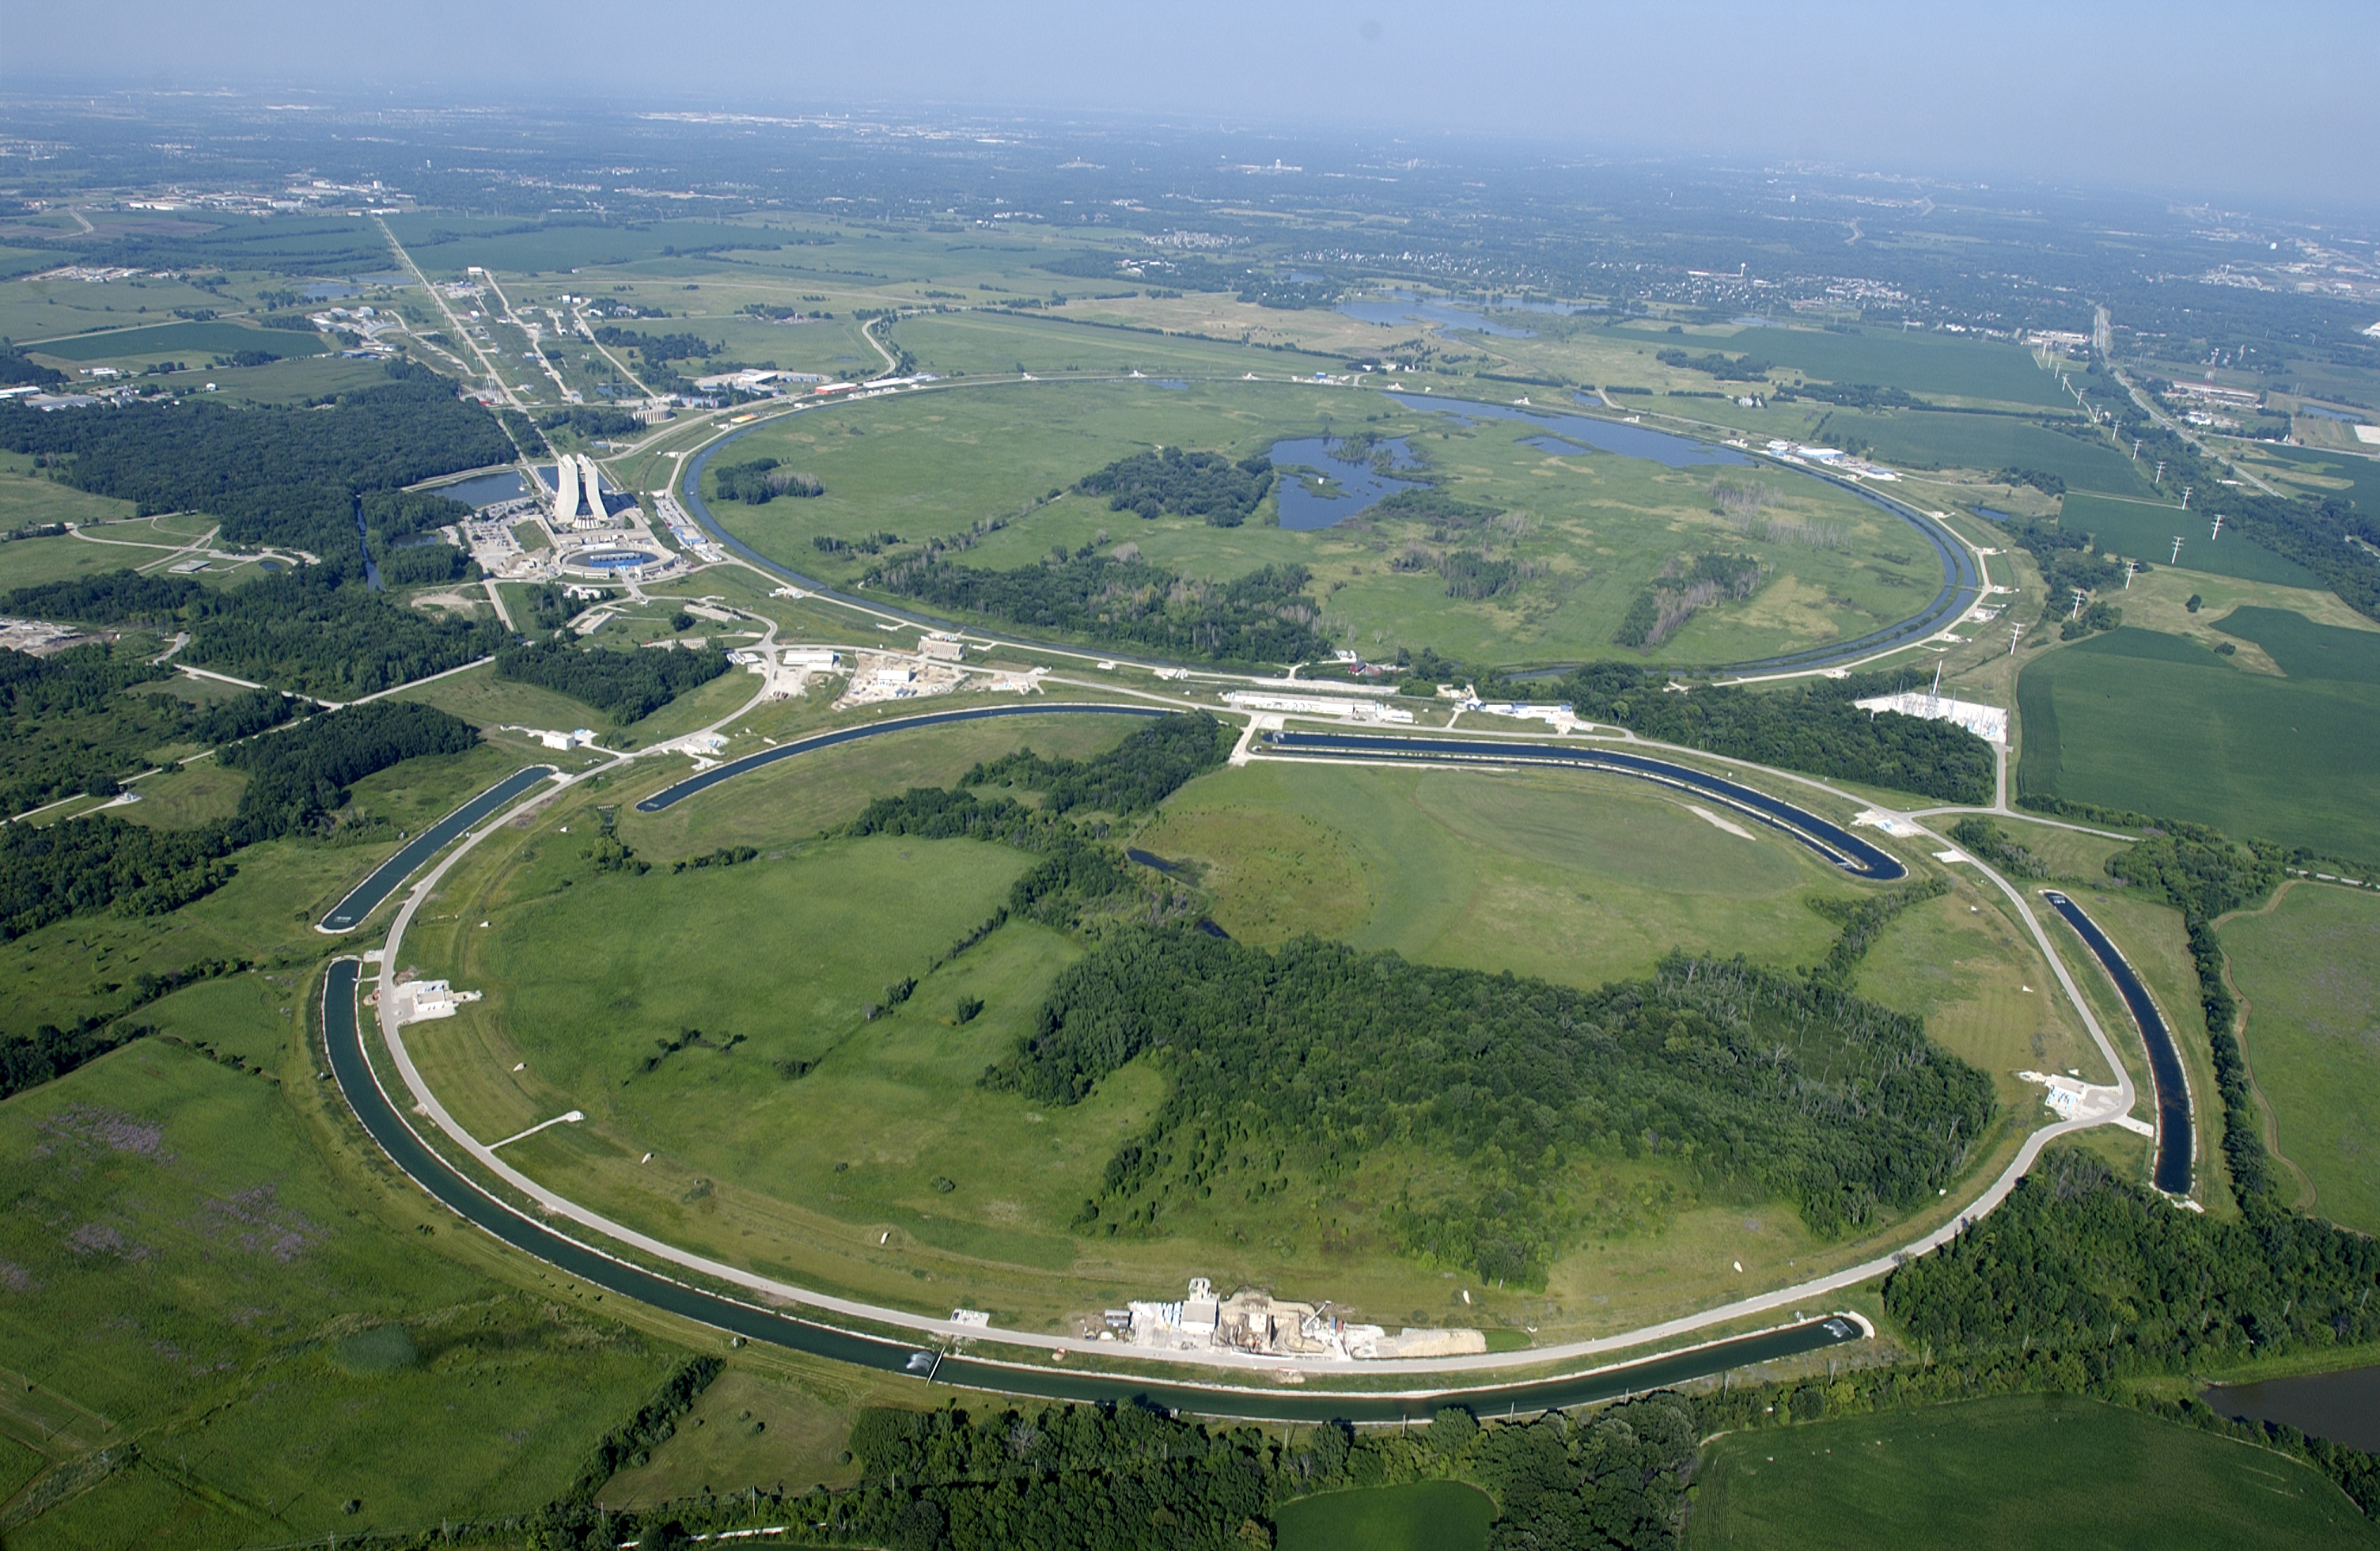
\includegraphics[width=\columnwidth]{chapter1/fermilab.jpeg}
    \caption{Aerial view of the Fermi National Accelerator Laboratory (FNAL) located in Batavia, IL, USA \cite{fermipic}.}
    \label{fig:fermia}
 \end{figure}

The Fermi National Accelerator Laboratory (FNAL), better known as Fermilab, has a long and rich history of designing, building, and operating high-energy particle accelerators. Ever since the founding director of Fermilab, Robert R. Wilson, envisioned the 400 GeV Main Ring back in 1967, Fermilab has been at the forefront of accelerator physics \cite{fermilab1,fermi50,tevatron}. The most famous accelerator project hosted by Fermilab has been the Tevatron, a proton-antiproton circular collider with a circumference of around 6.28 km. This machine took protons and antiprotons from smaller machines still in operation or repurposed as of 2024, e.g., the Recycler Ring. The Tevatron operated up until 2011, leaving an indelible legacy in the field of high energy and accelerator physics. Nostalgia aside, Fermilab still hosts a deluge of particle physics experiments connected to its main accelerator complex.      

Figure \ref{fig:fac} summarizes the current layout of the Fermilab Accelerator Complex. As of 2024, the Fermilab Accelerator Complex is composed of an $H^-$ source that connects to a linear accelerator, accelerating the ions to an energy of 400 MeV. This linear accelerator feeds to the first circular machine---the Booster---where protons are achieved and accelerated to an energy of 8 GeV. After the Booster, the protons are transported to the Recycler Ring (RR), which is the second circular machine. The Recycler Ring stores and stacks protons to increase the beam intensity delivered to the Main Injector (MI). This last circular accelerator is where protons are accelerated from an energy of 8 GeV to 120 GeV. Once at this energy, the protons are transported to the Neutrinos at the Main Injector (NuMI) experiment to create the world's most intense neutrino beam \cite{numi1}. Nevertheless, throughout the chain of accelerators, the beam is also delivered to many other experiments. Therefore, the facility has several modes of operation depending on the online experiments. A more detailed and technical study of the current Fermilab Accelerator Complex, focusing on the Recycler Ring, is given in Ch. \ref{sec:ch3}.   

\begin{figure}[H]
    \centering
    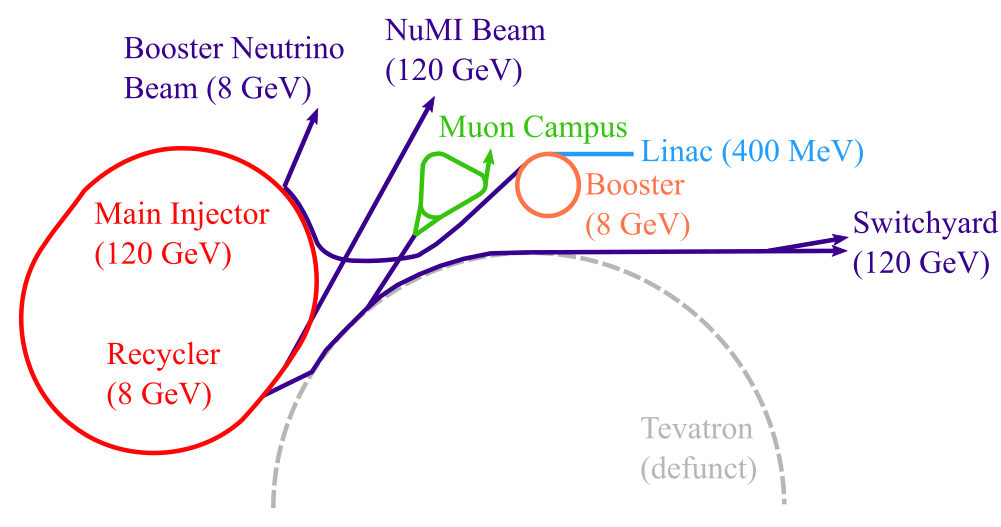
\includegraphics[width=\columnwidth]{chapter1/complex.png}
    \caption{Schematic layout of the Fermilab Accelerator Complex as of 2024. Original plot provided by R. Ainsworth, first published on Ref. \cite{rr1}.}
    \label{fig:fac}
 \end{figure}

\section{Outline}

The following thesis will explore the compensation of third-order resonances in the Fermilab Recycler Ring. Chapter \ref{sec:ch1} introduces the motivation behind this thesis work. Chapter \ref{sec:ch2} summarizes single particle dynamics with exponential Lie operators' help and introduces a relevant concept of collective beam dynamics: the space charge tune shift. This theoretical overview gives a segue into this thesis' Ch. \ref{sec:ch3}, where the Recycler Ring is introduced and described in detail. This chapter motivates the compensation of third-order resonances under the framework of the current and future operation of the RR. With the basic physics concepts and the description of the machine put in place, \hyperref[sec:ch4]{Ch. 4} describes in full detail the scheme and experiments developed to compensate for third-order resonances at low intensities. Before moving to explore the Recycler Ring at high intensities, Ch. \ref{sec:ch5} provides an interlude to show a series of experiments done at the CERN PS Booster. These experiments explore the use of advanced optimization algorithms to compensate for multiple resonance lines simultaneously. Coming back to Fermilab, Ch. \ref{sec:ch6} showcases the studies and experiments done at high intensities in the RR to understand the interplay between the compensation of resonance lines and space charge effects. Finally, Ch. \ref{sec:ch7} brings down the curtain by providing some general conclusions and future work stemming from this thesis.